\section{Methods}
\label{subsec:methods}

Firstly, technical terms specific to the domain are defined and briefly discussed.
Afterwards, the used methods are described in detail.
Concepts used in the approach by Cook and Diehl \cite{SNN} include \acfi{LIF} neurons, lateral inhibition, synaptic plasticity and homoeostasis, which are outlined in this section.

\newcommand\rbModel{Rate-based model}
\newcommand\sbModel{Spike-based model}
\subsection{Terms}
\label{subsec:terms}

In this section, technical terms specific to the domain are defined and briefly discussed.

\subsubsection{Spike trains}
are defined as multiple spikes.
\textcolor{red}{
They are encoded as a 1-bit array, where each entry indicates whether a spike (1) or no spike (0) occurred at a certain point in time.
}

\subsubsection{\rbModel{}}
According to \cite{spike_vs_rate} there are two central beliefs with regard to the question of how the neurons communicate with each other.
The firing rate of a neuron is an abstract measurement of the average number of spikes per unit (e.g. duration, neuron, trial).
The \rbModel{} believes that the firing rate captures most of the information, hence the timing of spikes is meaningless.

\subsubsection{\sbModel{}}
According to the \sbModel{}, the firing rate is not sufficient to describe the neural activity.
The spike timing defines spike trains and individual spikes.
As stated in \cite{spike_vs_rate}, the \rbModel{} assumption is stronger than the one of the \sbModel{}.

\subsubsection{Rate-based learning} uses backpropagation during training, but converts the \ac{ANN} to a \ac{SNN} (i.e. transfers trained weights) afterwards. 
According to \cite{SNN} and \cite{STDP_like} the usage of backpropagation is biologically unrealistic.


\subsection{\ac{SNN}'s methods}

\paragraph{\textbf{Input encoding}}
\acp{SNN} transmit information through spikes and thus, analogue values have to be encoded into spikes \cite{DIET_SNN}.
There are different types of encodings based on certain beliefs, 
for instance, those outlined in \autoref{subsec:terms}.
%in \autoref{subsubsec:communication}.

$60,000$ training examples and $10,000$ test examples of $28\times 28$ pixel images of the digits 0 to 9 compose the MNIST dataset used in the work of 
\authorsSNN{}, \authorsANNSNNconversion{} and \authorsRBMSNN{} \cite{SNN,ANN_SNN_conversion,RBM_SNN}.
There is a method to encode analogue values into spikes:
Inputs are Poisson spike trains, which are presented for 350ms.
The intensity of a pixel (0 to 255) is proportional to the firing rates (0 to $65.75 Hz$) of the neurons.
If the network does not react to the input, the maximum input firing rate is augmented until the neurons fire in the desired fashion. 

\vspace{-3mm}
\paragraph{\textbf{Poisson model of spike generation}}
%The timing of successive action potentials in biology can be modelled by stochastic processes, 
%due to the observed irregularity of interval lengths between spikes \cite{poisson_spike_generation}.
%The hypothesis that the generation of an individual spike is independent of the generation of others 
%is necessary to use Poisson processes to model spike trains.
A Poisson spike generator generates spikes according to a Poisson process \cite{poisson_spike_generation}.
%Different methods to generate spikes, which are either assigned to continuous time values or to discrete time bins,
% are outlined in \cite{poisson_spike_generation}.
 
\vspace{-3mm}
\paragraph{\textbf{Timing of spikes}}
The timing of spikes determines the type of synaptic changes \cite{LTP_D_bio}:
If multiple postsynaptic spikes occur close after presynaptic spikes, a \acfi{LTP} is induced, 
whereas repetitive postsynaptic spikes before the presynaptic ones lead to \acfi{LTD}.

\vspace{-3mm}
\paragraph{\textbf{Synaptic plasticity}}
Synapses play a crucial role in \ac{SNN} learning tasks such as recognition and computation \cite{Synaptic_plasticity}.
The term \textit{synaptic plasticity rules} is used for the different mathematical formulae realised in activity-dependent modification of synaptic weights.
There is a great variety of synaptic plasticity rules, ranging from abstract models to detailed models \cite{Synaptic_plasticity}.

Instances of abstract models include those based on the timing of spikes, such as pair-based \ac{STDP} models.
\autoref{eq:pair_based_weight_update} from \authorsSynapticPlasticity{}'s paper \cite{Synaptic_plasticity} shows the weight update of a pair-based \ac{STDP} model.
$\Delta t = t_{post} - t_{pre}$ is the time difference between the presynaptic spike $t_{pre}$ and the postsynaptic spike $t_{post}$.
If a postsynaptic spike arrives within the time window $\tau_+$ after a presynaptic one, potentiation occurs, i.e. the synaptic weight is increased. 
Analogously to induce depression the postsynaptic spike needs to precede the presynaptic one within time window $\tau_-$.
The amount of weight change depends on $\Delta t $ and the amplitude parameters $A^+$ and $A^-$.
%
\begin{equation}
    \centering
    \label{eq:pair_based_weight_update}
    \Delta w = \left\{
        \begin{array}{ll}
        \Delta w^+ = A^+ e^{\frac{-\Delta t}{\tau_+}}, & \text{if } \Delta t > 0 \\
        \Delta w^- = -A^- e^{\frac{\Delta t}{\tau_-}}, & \text{if } \Delta t \le 0 \\
        \end{array}
        \right.
\end{equation}
%
\autoref{fig:weight_change_time_dep} visualizes the concept of 
the weight modification dependence on the temporal relationship of the presynaptic and the postsynaptic spike.
%
\begin{figure}[htbp]
    \center
    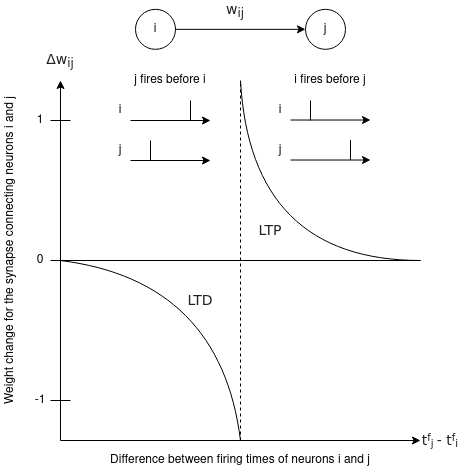
\includegraphics[width=0.4\textwidth]{pictures/weight_change_time_dep_altered.png}
    \caption{Weight modification depending on the time difference $\Delta t = t_j^f - t_i^f$ 
    between postsynaptic and presynaptic spike from \authorsSNNweightTime{}'s paper \cite{snn_weight_time}.
    The weight change $\Delta w$ is positive if the presynaptic spike precedes the postsynaptic one, 
    i.e. $\Delta t > 0$, analogously for $\Delta t < 0$.
    The size of $\Delta w$ depends on the size of $\Delta t$.}
    \label{fig:weight_change_time_dep}
\end{figure}

Other models, for instance, the \ac{TSTDP}, not only consider a single pair of presynaptic and postsynaptic spikes, 
but triplet combinations of spikes \cite{Synaptic_plasticity,STDP_triplet}.

Detailed models, on the other hand, may take into account state variables, such as membrane potential, 
accounting for more biophysically realistic models.
Changes in the synaptic weight of an instance of the \ac{SDSP} model depend on the postsynaptic membrane potential $V_{mem}$ and 
the calcium concentration $C(t)$ \cite{Synaptic_plasticity}.
The calcium variable is used to model the influence of the $Ca^{2+}$ level on activation neurons observed in biology \cite{STDP_hebbian}:
Presynaptic action potentials release neurotransmitters that bind to certain receptors and 
when the postsynaptic activities provide sufficient constant membrane depolarization, the $Ca^{2+}$ level rises \cite{Synaptic_plasticity}.
A large $Ca^{2+}$ rise is associated with \ac{LTP}, whereas modest $Ca^{2+}$ rise may result in \ac{LTD} \cite{STDP_hebbian}.
The calcium concentration $C(t)$  modification with regard to the temporal interplay of decay and incrementation is outlined in the work 
of \authorssimulationSTDP{} \cite{simulation_STDP}.
Whenever a presynaptic spike arrives, either potentiation of amount $a$ takes place, 
if the membrane potential $V_{mem}$ is higher than a certain threshold $V_{mth}$ and the 
calcium concentration $C(t)$ is within certain bounds, 
or depression of amount $b$\footnote{The origin and nature of $a$ and $b$ is not covered in \authorsSynapticPlasticity{}'s work \cite{Synaptic_plasticity}.}, analogously displayed in 
\autoref{eq:sdsp_weight_update} from the work of \authorsSynapticPlasticity{} \cite{Synaptic_plasticity}, occurs.
%
\begin{equation}
    \centering
    \label{eq:sdsp_weight_update} 
    W = 
    \left\{
    \begin{array}{ll}
        W + a, & \text{if } V_{mem} > V_{mth} \text{ and } \theta^l_{up} < C(t) < \theta^h_{up}\\
        W - b, & \text{if } V_{mem} \le V_{mth} \text{ and } \theta^l_{dn} < C(t) < \theta^h_{dn}
    \end{array}
    \right.
\end{equation}
%
If the conditions from \autoref{eq:sdsp_weight_update} are not satisfied or no spike arrives, 
the synaptic weight drifts towards either high or low synaptic weight asymptotes dependent on the weights at a specific time $t$ 
with respect to a threshold $\theta_W$ \cite{Synaptic_plasticity}.
The \ac{SDSP} approach models synaptic weight $W$ decay as displayed in \autoref{eq:sdsp_weight_decay} from \authorsSynapticPlasticity{}'s paper \cite{Synaptic_plasticity}.
%
\begin{equation}
    \centering
    \label{eq:sdsp_weight_decay}
    \frac{dW(t)}{dt} = 
    \left\{
    \begin{array}{ll}
        \alpha, & \text{if } W(t) > \theta_W\\
        - \beta, & \text{if } W(t) \le \theta_W\\
    \end{array}
    \right.
\end{equation}

Other detailed models, such as \ac{LCP} are outlined by \authorsSynapticPlasticity{} \cite{Synaptic_plasticity} 
and \authorssimulationSTDP{} \cite{simulation_STDP}.

\vspace{-3mm}
\paragraph{\textbf{Learning using \ac{STDP}}}
The synapses of the \ac{SNN} are trained using unsupervised \acfi{STDP}, which has been observed in a range of species from insects to humans \cite{STDP_hebbian}. 
The weight of a connection between two neurons models a synapse.
\ac{STDP} is a synaptic learning rule, which adapts weights of synapses according to their degree of causality \cite{STDP_like,multi_scale_STDP},
 i.e. how likely the input causes postsynaptic neuron excitation.
\ac{STDP} increases synaptic weight if the postsynaptic neuron reacts immediately after the presynaptic neuron fires \cite{object_detection_SNN}.
The goal of \ac{STDP} is to strengthen synapses of pre- and postsynaptic neuron pairs, 
whose postsynaptic neuron reacts immediately after the presynaptic neuron fires \cite{object_detection_SNN}.
If the postsynaptic neuron fires before the presynaptic one, the spike has another origin and thus, the synapse is weakened to disconnect the neurons.
\ac{STDP} can be considered the transposition of the Hebbian learning rule in a temporal context \cite{STDP_vis_feat}.
%
\begin{equation}
    \centering
    \label{eq:weight_update}
    \Delta w = \eta (x_{pre} - x_{tar})(w_{max}-w)^\mu
\end{equation}
%
\autoref{eq:weight_update} from \authorsSNN{}'s paper \cite{SNN} calculates the weight change after a postsynaptic spike arrives 
(i.e. the synapse's importance is changed according to its influence on the postsynaptic neuron).
$\eta$ is the learning rate, presynaptic trace $x_{pre}$ tracks the number of recent presynaptic spikes 
(decaying if no spike arrives, increased by one otherwise), 
$\mu$ is the dependence of the update on the previous weight and 
$x_{tar}$ is the target value of the presynaptic trace at the moment of the postsynaptic spike.
If $x_{tar}$ is high, i.e. many spikes arrived at the postsynaptic neuron, the weight will probably not be increased 
(especially if fewer spikes arrived at the presynaptic neuron indicated by  $x_{pre}$).

If multiple presynaptic and postsynaptic spikes arrive closely in time, there are different methods to compute the total weight change \cite{simulation_STDP}:
One could consider only nearest neighbour pairs of presynaptic and postsynaptic spikes, or sum up the weight changes for all pairs.

There are also other \ac{STDP} learning rules \cite{SNN,STDP_random}.
Some \ac{STDP} models rely on a teaching signal, which provides the right response \cite{STDP_like}.
Teaching signals are generated by Poisson spike generators.
A teaching signal is sent to the correct pool of neurons representing the class (i.e. digit) after a stimulus was presented in the training phase.
The goal of this approach is to make each neuron pool selective to one class of input.

\ac{STDP} focuses on the target object features, generally not learning the background, since they are usually too different to converge on them \cite{multi_scale_STDP,STDP_vis_feat}.
Hence, \ac{STDP} allegedly extracts informative and diagnostic features.

\vspace{-3mm}
\paragraph{\textbf{Neuron model}}
%\label{subsubsec:neuron_model}
In reality, a neuron fires if the membrane's potential $V$ crosses the membrane's threshold $\nu_{thresh}$.
After firing, the neuron's membrane potential is reset and within the next few milliseconds, i.e. the refractory period $t_{ref}$ \cite{RBM_SNN}, 
the neuron cannot spike again \cite{SNN}.
The model at hand displays similar behaviour as displayed in \autoref{fig:input_thres_output}.
%
\begin{equation}
    \centering
    \label{eq:membrane_vol_pot}
    \tau \frac{dV}{dt} = (E_{rest} - V) + g_e(E_{exc} - V) + g_i(E_{inh} - V)
\end{equation}
%
\autoref{eq:membrane_vol_pot} from \authorsSNN{}'s paper \cite{SNN} describes the membrane voltage 
(i.e. the value compared to the threshold $V_{thres}$ which determines whether the neuron fires) change over time constant $\tau$.
$E_{rest}$ is the resting membrane potential, $E_{exc}, E_{inh}$ are equilibrium potentials of excitatory and inhibitory synapses, 
and $g_e, g_i$ the conductances of excitatory and inhibitory synapses (i.e. the influence of respective synapses on membrane voltage of neuron) \cite{SNN}. 
The voltage decays (first parenthesis) and is influenced by the excitatory synapses 
adding to the voltage and the inhibitory synapses subtracting from the voltage.
%
\begin{figure}[htbp]
    \center
    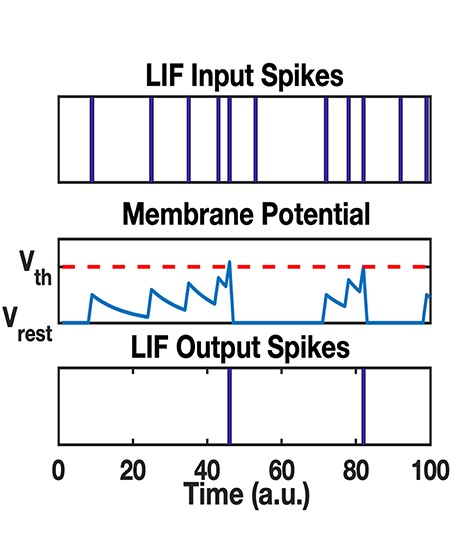
\includegraphics[width=0.3\textwidth]{pictures/input_pot_thres_output_altered.jpg}
    \caption{The \ac{LIF} neuron firing mechanism displayed in \authorsinputThresOutput{}'s work \cite{input_thres_output}.
    \ac{LIF} neurons integrate incoming spikes and decay otherwise.
    If the membrane potential $V$ crosses the threshold $V_{thres}$, the neuron fires and thus, 
    enters a refractory period at the resting membrane potential.}
    \label{fig:input_thres_output}
\end{figure}

\vspace{-3mm}
\paragraph{\textbf{Synapse model}}
%\label{subsubsec:synapse_model}
The synapse's conductance $g_e$/$g_i$ ($e$ excitatory, $i$ inhibitory) models the influence of a presynaptic neuron on another neuron.
If a presynaptic spike arrives at the synapse the weight $w_{i,j}$ between neuron $i$ and neuron $j$ is added to $g_e$/$g_i$.
Otherwise, $g_e$/$g_i$ is decaying.
%
\begin{equation}
    \centering
    \label{eq:exc_conductance}
    \tau_{g_e} \frac{dg_e}{dt} = - g_e
\end{equation}
%
The decay of $g_e$ ($g_i$ analogously) is computed using \autoref{eq:exc_conductance} from \authorsSNN{}'s paper \cite{SNN}.
The change over time constant $\tau$ is an exponential decay.

\vspace{-3mm}
\paragraph{\textbf{\ac{LIF} neurons}}
The \ac{LIF} neuron is a simple, yet biologically plausible model of a spiking neuron \cite{RBM_SNN}.
As depicted in \autoref{eq:membrane_vol_pot}, the membrane potential/ voltage $V$'s current leaks out of the neuron 
(i.e. decays without incoming spikes over time).
Due to the exponential decay, these neurons are called \ac{LIF} neurons.
%\acp{LIF} neuron states are only updated, i.e. fire or not, when a spike arrives \cite{RBM_SNN} (in event-based networks).

\vspace{-3mm}
\paragraph{\textbf{Lateral inhibition}}
Since every inhibitory neuron is connected to all excitatory neurons except the one it is already connected to, 
whenever a spike is triggered in an excitatory neuron all inhibitory neurons receive a spike as well.
Hence, neurons that did not fire are inhibited and thus, lateral inhibition and a soft winner-take-all mechanism are created \cite{SNN}.

\vspace{-3mm}
\paragraph{\textbf{Homoeostasis}}
In order to ensure the neurons have a similar firing rate, the \eN{}'s membrane threshold is calculated by $\nu_{thresh} + \theta$, 
where $\theta$ is increased every time the neuron fires and decays exponentially otherwise.
Since the membrane potential is limited to $E_{exc}$ a neuron stops firing when its membrane threshold is higher than the maximum membrane potential.

This technique countersteers the effect of inhomogeneity of the input and lateral inhibition.

\vspace{-3mm}
\paragraph{\textbf{Competitive Learning}}
The goal of the \ac{SNN}-model is to train its neurons to represent prototypical inputs or an average of similar inputs \cite{SNN}.
To achieve this goal, the weights of spiking neurons are adapted to become more similar to the input.
Lateral inhibition prevents too many neurons from spiking and thus, prevents them from becoming too similar in the course of adapting to the input.
This results in the receptive fields of the neurons exploring the input space.
To ensure that an approximately constant number of neurons' receptive fields is similar to an input, 
homoeostasis guarantees similar firing rates among the neurons.
The learning procedure is similar to k-means-like learning algorithms \cite{SNN}.
Hence, increasing the number of neurons may result in at most 95-97 \% accuracy.

\vspace{-3mm}
\paragraph{\textbf{Training}}
In order to allow all variables to decay there is a 150ms phase without any input between images.

\vspace{-3mm}
\paragraph{\textbf{Testing}}
First the learning rate $\eta$ is set to zero to appoint the neuron's threshold.
After that, the training set is presented once more.
The highest response among the ten-digit classes is used to assign a class to each neuron, i.e. labels are used.
The predicted value for an input is the class whose neurons have the highest average firing rate.
The classification accuracy is determined on the MNIST test set.